\documentclass[10pt]{article}

\usepackage{graphicx}
\usepackage{ifthen}
\input{/home/donma/Documents/src/ib/AITrading_24_7/StepByStep/aitrading-preamble.tex}
\usepackage[nameinlink,capitalise]{cleveref}

\newboolean{draftmode}
\setboolean{draftmode}{false}
\input{/home/donma/Documents/Pointer/TexCompilationTools/SumCounterControl.tex}
\input{/home/donma/Documents/Pointer/TexCompilationTools/SumControl.tex}
\input{/home/donma/Documents/Pointer/TexCompilationTools/SumAuthorControl.tex}

\setlength{\headheight}{14pt}
\setlength{\headwidth}{\textwidth}
\setcounter{tocdepth}{1}
\fancyhead[L]{\small\textcolor{uablue}{Weekly Research Update}}
\fancyhead[R]{\small\textcolor{uablue}{September 15, 2026}}
\hypersetup{
  colorlinks=true,
  linkcolor=uablue,
  urlcolor=uablue,
  citecolor=accent,
  filecolor=accent,
  menucolor=uablue,
  linktoc=all,
  breaklinks=true,
  pdftitle={Weekly Research Update for September 15, 2026},
  pdfsubject={Bi-objective intersection paper revision: component rebuild and first production attempt},
  pdfauthor={Muting Don Ma}
}

\newcommand{\statusdone}{\textcolor{definitiongreen}{\textbf{Completed:}}\ }
\newcommand{\statusprogress}{\textcolor{uablue}{\textbf{In progress:}}\ }
\newcommand{\statusblocked}{\textcolor{accent}{\textbf{Blocked:}}\ }
\newcommand{\projectline}[1]{%
  {\small\noindent\textbf{Name:} Muting (Don) Ma\hfill
    \textbf{Project:} #1\hfill
    \textbf{Date:} September 15, 2026\par}
  \vspace{0.18em}\hrule\vspace{0.42em}}
\newenvironment{tightitems}{%
  \begin{itemize}[leftmargin=1.15em,label=\textcolor{uablue}{\scriptsize$\bullet$},
    topsep=0.10em,itemsep=0.16em,parsep=0pt,partopsep=0pt]}{\end{itemize}}
\newcommand{\artifact}[2]{\href{#1}{#2}}

\begin{document}

\hypersetup{pageanchor=false}
\begin{titlepage}
\thispagestyle{empty}
\vspace*{0.16\textheight}
\begin{center}
  {\Huge\bfseries\textcolor{uablue}{Weekly Research Update}}\\[0.8em]
  {\Large Single Project Progress Report}\\[2.2em]
  {\large Muting (Don) Ma}\\[0.45em]
  {\large September 15, 2026}\\[3em]
  \fcolorbox{uablue}{uablue!4}{%
    \parbox{0.76\textwidth}{\centering\large
      Bi-objective Intersection Paper Revision\\[0.6em]
      Component Rebuild and First Production Attempt}}
  \\[3em]
  \small Public artifacts:
  \href{https://github.com/mutingma123/OpenProjects}{OpenProjects repository}

  \vspace{2.2em}
  \sumpara The front-page note states the report's scope and its evidence base. \sumparaend
  \parbox{0.80\textwidth}{\small\centering
    \fin This report covers one project, the revision of the bi-objective connected and automated vehicle intersection manuscript, since the September 2, 2026 meeting. \fine
    \fin Its five sections follow the requested update format, and every claim traces to the commit history of the manuscript repository, the new runtime package, and the retired legacy codebase. \fine
    \fin The referenced works follow the five sections. \fine}
\end{center}
\end{titlepage}
\hypersetup{pageanchor=true}

\clearpage
\pagenumbering{roman}
\setcounter{page}{1}
\tableofcontents
\clearpage

\pagenumbering{arabic}
\setcounter{page}{1}

\section{Current Objective}
\label{sec:objective}
\projectline{Bi-objective Intersection Paper Revision}

\sumpara The context fixes the decision problem and the scope of the present revision. \sumparaend
\noindent\textbf{Context.}
\fin At a reservation-based intersection, the manuscript schedules connected and automated vehicles by trading average speed against priced collision risk \cite{ma2025socio}. \fine
\fin The revision answers the six experiments requested at the August meeting, so the evidence, not the exposition, is the deliverable. \fine
\fin Its benchmark set carries six controller classes, with the published speed-maximization method mapped onto the delay-only class \cite{ma2023speed}. \fine

\subsection{Objective}
\label{sec:objective:statement}

\sumpara The objective is stated in one sentence, as the update format requires. \sumparaend
\begin{tightitems}
  \item \fin Deliver the six requested experiments as schedules that are certified optimal, independently validated, and reproducible from saved artifacts. \fine
\end{tightitems}

\section{Progress Since the Last Meeting}
\label{sec:progress}

\sumpara The progress separates the completed rebuild from the production run that is now blocked. \sumparaend
\begin{tightitems}
  \item \fin \statusdone Rebuilt the study as eleven component contracts in the manuscript repository and a matching \texttt{biobj} runtime package, retiring the legacy BiCAVO codebase after its audit against the six experiment plan. \fine
  \item \fin \statusdone Replaced the rear-end time-to-collision surrogate with a priced contact probability, replaced the thousand draw replay with exact expectations at each timing error width, and widened initial following gaps to hold modeled contact risk at or below 0.1 percent. \fine
  \item \fin \statusblocked The first production campaign ran twelve workers for 2 hours and 52 minutes and was stopped: 14 of 4,410 report rows were saved, and 13 of those 14 fail the independent validator. \fine
\end{tightitems}

\section{Key Result or Lesson}
\label{sec:key}

\sumpara The key result names the contradiction inside the saved rows and the cost of solving to a zero gap. \sumparaend
\begin{tightitems}
  \item \fin Every saved solve is certified optimal at a zero optimality gap, yet recounting its own trajectory places two vehicles in one conflict cell and raises the crossing count by 2 to 6, so the model's occupancy constraints and the validator's recount do not agree. \fine
  \item \fin Solving to a zero gap does not scale: the launched settings project 802 days to finish the design, with a 10th to 90th percentile range of 654 to 1,125 days. \fine
  \item \fin Restricting the campaign to the five eight-vehicle cases projects 43 days, and a one hour limit per solve projects 10 days, which makes the gap policy, not the hardware, the binding choice. \fine
\end{tightitems}

\begin{figure}[!ht]
  \centering
  \href{https://github.com/mutingma123/OpenProjects/blob/main/BiObjectivePaperRevision/Figures/ProductionAttemptStatus.png}{%
    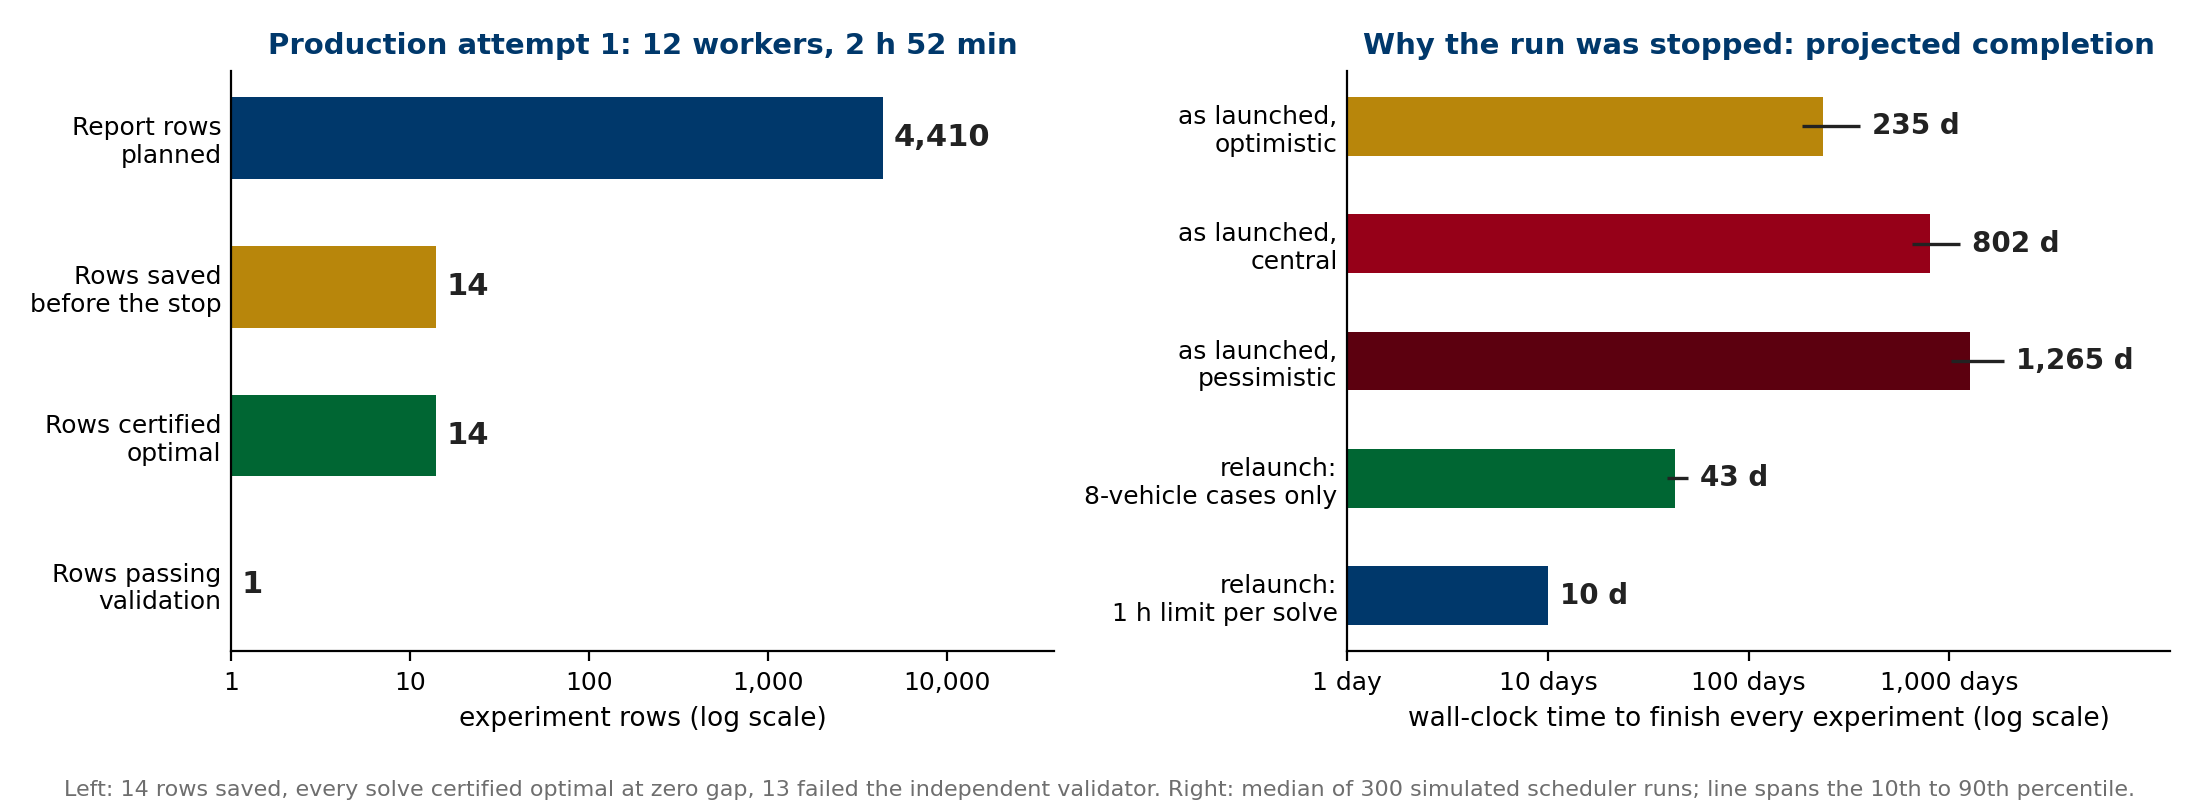
\includegraphics[width=0.96\textwidth]{../../BiObjectivePaperRevision/Figures/ProductionAttemptStatus.png}}
  \caption{Saved rows of the first production attempt and the projected time to finish the full design.}
  \label{fig:production-status}
\end{figure}

\section{Input Needed from Dr.\ Gong}
\label{sec:input}

\sumpara The requested input fixes the reconciliation target and the solver policy for the large cases. \sumparaend
\begin{tightitems}
  \item \fin Should the reconciliation in \cref{sec:key} change the model's cell occupancy constraints, or the validator's recount of the saved trajectory? \fine
  \item \fin Should the sixteen and twenty-four vehicle cases carry a per-solve time limit with reported bounds and gaps, or remain at a zero gap at the cost of the schedule in \cref{fig:production-status}? \fine
\end{tightitems}

\section{Before the Next Meeting}
\label{sec:next}

\sumpara The deliverables repair the disagreement before any campaign is relaunched. \sumparaend
\begin{tightitems}
  \item \fin Reconcile occupancy and crossing counts between the model and the validator at the production 0.1 second time step. \fine
  \item \fin Relaunch the five eight-vehicle cases, writing rows to local disk and copying finished rows to the synced folder with retries. \fine
  \item \fin Report per-row bounds, gaps, and validation outcomes for every relaunched row. \fine
\end{tightitems}

\vspace{0.6em}
{\footnotesize\textbf{Public artifacts:}
\artifact{https://github.com/mutingma123/OpenProjects/tree/main/BiObjectivePaperRevision}{project folder};
\artifact{https://github.com/mutingma123/OpenProjects/tree/main/BiObjectivePaperRevision/Figures}{selected snapshot}.\par}

\clearpage
\phantomsection
\addcontentsline{toc}{section}{References}
\begin{thebibliography}{9}
\small

\bibitem{ma2025socio}
\fin M. Ma and M. Yavuz, ``Socioeconomic Tradeoff on Connected and Automated Vehicles Scheduling at a Reservation-based Intersection,'' Social Science Research Network, 2025. \fine
\href{https://doi.org/10.2139/ssrn.5372729}{doi:10.2139/ssrn.5372729}.

\bibitem{ma2023speed}
\fin M. Ma and Z. Li, ``A Speed-Maximization Trajectory Optimization Model on a Reservation-Based Intersection Control System,'' \textit{Transportation Research Part C: Emerging Technologies}, vol. 154, art. 104266, 2023. \fine
\href{https://doi.org/10.1016/j.trc.2023.104266}{doi:10.1016/j.trc.2023.104266}.

\end{thebibliography}

\end{document}
